\documentclass{bmvc2k}

%% Enter your paper number here for the review copy
%\bmvcreviewcopy{??}

\title{Object-Centric Spatio-Temporal Pyramids for Egocentric Activity Recognition}

% Enter the paper's authors in order
% \addauthor{Name}{email/homepage}{INSTITUTION_CODE}
\addauthor{Tomas McCandless}{tomas@cs.utexas.edu}{1}
\addauthor{Kristen Grauman}{grauman@cs.utexas.edu}{1}

% Enter the institutions
% \addinstitution{Name\\Address}
\addinstitution{
 Department of Computer Science \\ 
 University of Texas at Austin
}

\runninghead{McCandless, Grauman}{Object-Centric Spatio-Temporal Pyramids}

% Any macro definitions you would like to include
% These are not defined in the style file, because they don't begin
% with \bmva, so they might conflict with the user's own macros.
% The \bmvaOneDot macro adds a full stop unless there is one in the
% text already.
\def\eg{\emph{e.g}\bmvaOneDot}
\def\Eg{\emph{E.g}\bmvaOneDot}
\def\etal{\emph{et al}\bmvaOneDot}

%------------------------------------------------------------------------- 
% Document starts here
\begin{document}

\maketitle

\begin{abstract}
	Egocentric video and wearable computing have become increasingly
	prevalent in the past decade, resulting in a huge explosion in the amount
	of available video content. In this paper, we present a novel approach for
	egocentric activity recognition using the UC Irvine ADL (Activities of Daily Living)
	dataset \cite{Ramanan12}.  
  Existing work in activity recognition uses predefined binning schemes,
  which may fail to capture important spatio-temporal relationships between
  features.
  We propose to partition video clips into sets of
	3-dimensional cuboids based on many different multi-level randomized partitioning
	schemes, then concatenate object histograms
	over multiple levels to form feature vectors which we then use to train a pool
	of weak SVM classifiers. 
	Finally, we use a boosting algorithm to learn which partitioning schemes are
  most discriminative and form a
	final strong classifier with accuracy that improves upon the current state of
	the art. Our main novel contribution is a method for
	creating biased partition schemes based on observed distributions of
	active object locations across each spatial and temporal dimension of the video clips.
  We found that partitions which cut through spatio-temporal regions that
  tend to contain active objects are often more discriminative than
  unbiased partitions and 
  partitions that cut around such active object regions.
\end{abstract}

%------------------------------------------------------------------------- 
\section{Introduction}
	Activity recognition is becoming an increasingly canonical problem in
	computer vision as researchers are beginning to explore the domain more
  thoroughly and several relevant datasets have been released 
  \cite{Schuldt04, Rodriguez08, Fathi11, Ramanan12}. 
	% past datasets scripted activities
	Datasets geared towards activity recognition in the past have often
	consisted of actors performing scripted activities in a static and at
  times artificial environment \cite{Schuldt04}. However, in order to develop robust and effective
	recognition methods, we need datasets that are more organic in the sense that they
	depict unscripted activities occurring in a natural environment such as a home or
	apartment.

	% application to life logging
	A robust and accurate method for egocentric activity recognition would have 
	many useful practical applications. For instance,
	a recent trend in wearable computing is so-called life logging which can
	assist patients suffering from memory loss \cite{Sellen07}. 
	A robust egocentric activity recognition
	system could automatically tag video clips with types of activities,
	thus allowing the user to, for
	example, quickly find all clips recorded in the past that depict making tea.
	
  Egocentric activity recognition in a daily living context differs from
  non-egocentric activity recognition because activities can have long-term
  temporal dependencies and actions can be interrupted by other actions. For
  example, a user might wash a few dishes while waiting for a cup of tea
  to brew. The familiar bag-of-words approach can be used to aggregate space-time
  features with reasonable performance, but ultimately falls short because it
  fails to capture temporal dependencies between features.
  The pyramid is a well-known extension of a pure bag-of-words model that encodes spatial
  relationships between features by recursively subdividing images or video and extracting 
  features from each spatial bin \cite{Lazebnik06}, yielding impressive
  results across a range of applications.
  
  Existing work in egocentric activity recognition has shown that activities
  are well-defined by the types of objects that are interacted with by users
  during particular actions \cite{Ramanan12}. 
  Previous work in egocentric activity recognition has often employed a single strict
  hand-coded partition scheme \cite{Ramanan12}, which may not be particularly robust to
  inter and intra-class variation. The work of \cite{Laptev08} uses multiple
  candidate spatio-temporal grids for the task of activity recognition (but
  not in an egocentric setting), however each grid is predefined and only 24
  possible
  candidate grids are considered. With a small pool of schemes for imposing spatial
  information, the most discriminative space-time relationships between features may not be 
  captured. The work presented in \cite{Kovashka10}
  describes an effective state-of-the-art method for learning the shapes of spatio-temporal
  regions on a per-class basis, but makes use of lower-level features such as
  optical flow, rather than object locations, and
  is not applied in an egocentric setting.

  Spatial pooling of features in a learned way for object recognition in 2D images
  has been thoroughly
  explored \cite{Sharma11}, but to our knowledge there has been little work
  on learning the best way to pool spatio-temporal features in video.
  
  Our proposed method, however, builds on existing work by creating a large number
  of candidate partitioning schemes in a randomized way. 
  We then pool spatio-temporal features in a
  learned way, using a boosting algorithm to select those partitioning schemes which are most discriminative.
  Our main novel contribution is
  the ability to bias the randomization step such that 
  resulting partition schemes have a high probability of cutting through or around
  spatio-temporal regions which are known to tend to contain active objects.
  We call pyramids generated according to this method object-centric
  pyramids.
  We found that partitioning schemes that have a larger number of levels and
  are biased to cut through regions known to contain active
  objects are often the most discriminative.
  We evaluate the performance of our method using a cross-validation
  experiment and found that our method using object-centric pyramids improves
  upon the current state of the art.

%-------------------------------------------------------------------------
\subsection{Related Work}


	In \cite{Laptev08}, Laptev \etal investigate automatically aligning movie scripts with
	video for the purpose of annotating human actions, and achieve 91.8\%
  accuracy on the KTH dataset. 
  Previous work on spatial pyramids \cite{Bosch07, Lazebnik06} is
  extended
  by defining the spatio-temporal pyramid representation of video clips, but uses a
  relatively small number of predefined schemes for spatio-temporal binning,
  which may fail to capture important spatio-temporal relationships between
  features. There are 6 possible spatial grids and 4 temporal binning
  schemes, resulting in a total of 24 possible spatio-temporal partition
  schemes. 
	
	In \cite{Marszalek09}, Marszalek \etal released a novel dataset based on
	Hollywood movies that contains twelve types of activities and ten
	different classes of scenes. The main contribution of this paper is based
	on the observation that the visual content of a human's environment can
	impose useful constraints on the type of activity occurring. For instance,
	food preparation activities frequently occur in a kitchen environment. 
	
	In \cite{Fathi12}, Fathi \etal focus on the relationship between gaze and
	activity recognition in an egocentric setting and develop methods to
	predict activity given gaze, gaze given activity, and both
	activity and gaze given neither. The activities in this
	published dataset are primarily related to food preparation. 
	
	The main work related to our own is that carried out in \cite{Ramanan12}. 
	In this work the ADL dataset is introduced as well as detailed analysis of
	performance of several different classifiers. 
	\begin{figure}[t]
		\begin{center}
			%\fbox{\rule{0pt}{2in} \rule{0.9\linewidth}{0pt}}
			  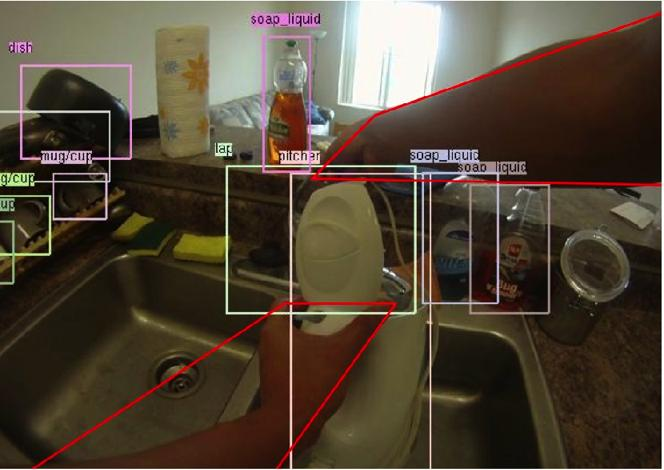
\includegraphics[width=0.7\linewidth]{figures/thumbnail.jpg}
		\end{center}
    \caption{An example frame from the ADL dataset with annotations for hand
    position and detected objects} 
				\label{fig:long}
				\label{fig:onecol}
	\end{figure}
  Composite object models are developed for the purpose of object detection. 
  These models take advantage of the fact that objects can have vastly
  different appearances when they are being interacted with. For example, a
  refrigerator or microwave has a different appearance when it is open and
  being interacted with. 
  A comparison of the well-known bag-of-words approach with a strict
  predefined
  2-level temporal pyramid using both space-time interest points and the
  results of the part-based object detectors is presented. The temporal pyramid makes 
  a single cut along the temporal dimension and no cuts along the
  spatial dimensions, but is simple, easy to implement, and outperforms a 
  classifier trained on bag-of-words histograms. The use of detected objects as
  features offers impressive improvement over using space-time interest points
  (STIP).
	The crucial contribution of
	\cite{Ramanan12} is that egocentric activity recognition is ``all about
	the objects'', particularly the objects being interacted with, as
	recognition accuracy increases dramatically when locations of active
  objects in addition to passive objects are used as features. 

	The video collected for the ADL dataset is available in a temporally
	presegmented format; each video has been segmented into clips depicting
	activities. Egocentric video is captured as a continuous stream, and thus
  a pre-processing step of temporal segmentation into discrete events is
  required. There is a large amount of literature on temporal segmentation
  of video. For instance, work presented in \cite{Lee12} includes a method for
	automatic temporal segmentation of egocentric video into events.
  
	Our algorithm is inspired by the work of \cite{Jiang12}, which uses a
  a version of the SAMME Ada-boost algorithm \cite{Zhu06}
  with randomized spatial pyramids for 2D images, 
	leading to increased robustness to intra-class variation based on results
  from benchmarks on three publicly available datasets. However, in contrast
  to our own work, the randomized pyramids are not biased in any way. 
	
	% work from other researchers on segmentation
	% work from other researchers on activity recognition with other modes of
	% sensor data

\section{Approach}

	Our boosting algorithm takes as input a collection of labeled training videos
	and a pool of candidate partition patterns. We use the output of the
  aforementioned object detectors trained on composite object models as our features to be
  pooled.
  We train a separate ``weak''
  multi-class SVM 
  (using LIBSVM \cite{Chang11})
	classifier on the feature vectors resulting from representing the training
	data using each candidate partition pattern $\theta$. We set a weight
  $w_i$ for each
	training point $p_i$ that is inversely proportional to the number of points
	with the same class as $p_i$. Giving larger weights to training examples of
  infrequently occurring actions helps to mitigate any bias resulting from imbalanced
  training data.
  During each round of boosting we select the
	candidate partition $\theta_j$ that is most discriminative (has minimum
  weighted training
	error, which is computed as the dot product between the weight vector $w$
  and an indicator of incorrect classifications using $f_\theta$)
  Next, we compute a weight for $\theta_j$, and compute accuracy for the
	current version of the final strong classifier, which maximizes a weighted
  sum of classifications produced by each weak classifier.
	We set the number of boosting rounds to 30.\\

	\noindent\textbf{Algorithm 1:} Training RSTP Classifier via Boosting \\
	\textbf{INPUT:} 
	\begin{itemize}
		\item $N$ labeled training videos $\Phi = \{(V_i, c_i)\}_{i=1}^N$
		\item A pool of $M$ partition patterns $\Theta = \{\theta\}$
	\end{itemize}
	\textbf{OUTPUT:}
	\begin{itemize}
		\item A strong video classifier $F$. For an unlabeled video $V$, 
			$c=F(V)$ is the predicted label for $V$.
	\end{itemize}
			\begin{enumerate}

				\item For each $\theta \in \Theta$:
					\begin{itemize}
            \item Compute the representations of each $V_i \in \Phi$ using $\theta$
						and train a multi-class classifier (SVM) $f_\theta$ on the
            resulting feature vectors.
					\end{itemize}

				\item Initialize:
					\begin{itemize}
						\item A weight $w_i = \frac{1}{C N_{c_i}}$ for each video clip,
							where $N_{c_i}$ is the number of videos with label $c_i$,
              and $C$ is the number of distinct labels in the training data.
						\item Current iteration number $j=0$.
						\item Current accuracy $\sigma_j = 0$.
					\end{itemize}

				\item For each round of boosting:
					\begin{itemize}
						\item Increment $j$.
						\item Re-normalize the weight vector:
              \begin{center}
              $\forall i, w_i = \frac{w_i}{\Sigma_i^N w_i}$.
              \end{center}
					  \item For each pattern $\theta$,
              compute its weighted classification error:
              \begin{center}
              $e_\theta = w \cdot \mbox{\textbf{I}}(f_\theta(V) \neq c)$
              \end{center}
						\item Choose the pattern $\theta_j$ with minimum weighted
              classification error $e_j$.
						\item Compute the weight for $\theta_j$:
              \begin{center}
              $\alpha_j = \mbox{log} \frac{1 - e_j}{e_j} + \mbox{log}(C-1)$
              \end{center}
						\item Update the weight vector:
              \begin{center}
							$w_i = w_i \cdot \mbox{exp}(\alpha_j \cdot
							\mbox{\textbf{I}}(f_{\theta_j}(V_i) \neq c_i))$.
              \end{center}
						\item Generate the current strong classifier:
              \begin{center}
							$F(V) = \mbox{argmax}_c \Sigma_{m=1}^j \alpha_m \cdot
							\mbox{\textbf{I}}(f_{\theta_m}(V) = c)$
              \end{center}
					\end{itemize}

			\end{enumerate}
	
	The original version of the SAMME algorithm has each weak classifier
	$f_\theta$ trained on
	a randomly sampled subset of the training examples, but we train each of
	our weak classifiers on the full training dataset.

  \subsection{RSTP Implementation}
	We use k-d trees to represent randomized partition schemes. Each level in the tree
	represents a set of cuts along a certain dimension, and we generate cuts
  for subsequent levels in the tree.
  in a round-robin manner over dimensions $(x, y, t)$. Cuts for child nodes are generated independently, and each cut is axis-aligned
  (we incorporate random shifts, but not random rotations).
  To construct a partition scheme that is easily applicable to videos of
  arbitrary size, we consider
  partitioning an ``idealized'' video clip that has all dimensions normalized
  to length 1. To generate a single cut we sample a random number from a
  distribution subject to any constraints imposed by ``parent cuts'' and use
  this as a randomized offset for an appropriate axis-aligned plane. To
  construct an unbiased partition scheme we sample from a uniform
  distribution.
  
  To represent a video clip as a randomized spatio-temporal pyramid (RSTP)
  using a particular partition scheme we use the output of object detectors
  trained in \cite{Ramanan12}, which gives bounding boxes and object
  labels for each extracted frame. We compute histograms of detected
  objects for each individual level in the pyramid,
  where level 0 is the entire video clip volume and level $i$ is all the
  cells of depth $i$ in the k-d tree. 
  Note that level $i$ has $8^i$ leaf
  cells. To form the final RSTP representation, we concatenate the
  histograms computed for each level to form a single feature vector.
  We can choose whether or not to include detected active objects when
  forming an RSTP representation of a video clip, however taking active
  objects into account gives a substantial improvement to overall
  classification accuracy.
  
  \subsection{Object-Centric Cuts (OCC)}
  The key novel contribution of our work is the ability to create
  meaningfully biased partition schemes that tend to be more discriminative
  than unbiased partition schemes.
  To accomplish this, we replace the uniform distribution with a discrete
  approximation of the distribution of active objects across each dimension
  $(x, y, t)$
  and otherwise proceed normally.

\begin{figure}
  \begin{center}
\begin{tabular}{cc}
\bmvaHangBox{\fbox{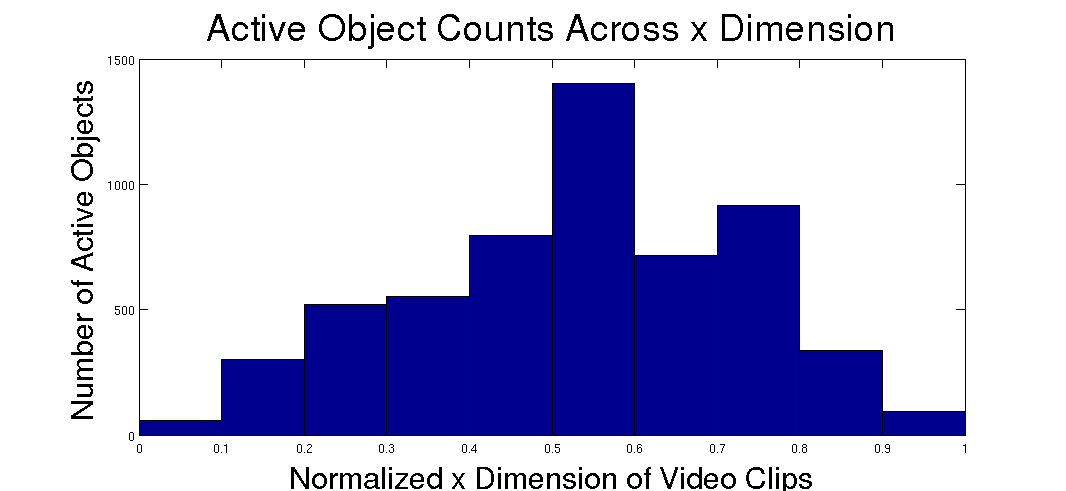
\includegraphics[width=5.9cm]{figures/active_obj_distr_x.png}}}&
\bmvaHangBox{\fbox{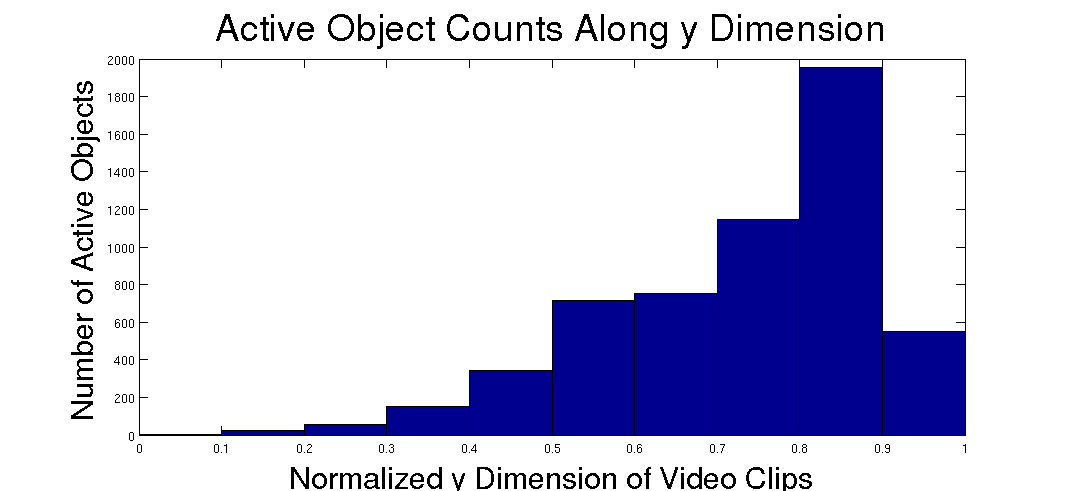
\includegraphics[width=5.9cm]{figures/active_obj_distr_y.png}}}\\
(a)&(b)
\end{tabular}
		   \caption{Histograms of detected active objects across the $x$ and
       $y$ spatial dimensions of training data. Active objects tend to appear in the lower
     center field of view. There is a slight bias favoring the
   right side of the field of view because many users are right-handed. }
\label{fig:teaser}
  \end{center}
\end{figure}
	
	From figure 2 we see that active objects often tend to occur in the lower center
	of the field of view. This conforms to our expectations, because
	the active objects are close to the hands which are in the lower field of
	view from an egocentric perspective. Active objects tend to occur on the
  right side of the field of view slightly more often because a large
  percentage of users are right-handed. Since different clips can have
  varying lengths with respect to time, we normalize the length of each
  video clip to 1 and consider relative temporal locations of active
  objects. The distribution of active objects
  across the temporal dimension is nearly uniform. When generating a biased
	partition scheme, we can choose to prefer splits that cut around regions that tend to
	contain active objects (denoted as bias type 2), or we can choose to prefer 
	splits that cut through regions that tend to contain active objects (denoted as bias type 3). 
	We denote by bias type 1 the method of using uniform
	distributions to generate partitions. For biased partitions, we generate
  the first split along each dimension according to a weighted distribution
  corresponding to the histograms of observed active object regions in the training data,
  and we generate all subsequent child cuts using a uniform distribution.
  We do not consider locations of passive objects at all during the
  generation of biased partition schemes. Since active objects are located
  in close spatial proximity to hands, creating biased partition schemes can
  be interpreted as implicitly taking into account information about hand
  locations.
  
  Figure 3 depicts an example 3-level partition scheme created using bias
  type 3. The salient feature to note is that visible splits along the $y$
  dimension correspond to the observed distribution of active objects along
  the $y$ dimension.

\section{Results}
  The ADL dataset consists of hundreds of egocentric video clips
	(roughly 10 hours of video in total) collected from 20 people performing
	18 types of unscripted actions in their own homes. These naturally
  occurring
  actions are often related to hygiene or food preparation and are more
  varied than actions presented in previous datasets such as that of \cite{Fathi11}.
  There are 26 different 
	types of detected objects, including 5 active and 21 passive objects. 
  Object detectors are trained on videos from the
  first 6 people and tested on the videos from the remaining 14 people.
  
	\begin{table}
		\begin{center}
			\begin{tabular}{|l|c|}
				\hline \hline
        label & activity type \\
        \hline
        1 & combing hair \\
        \hline
        2 & make up \\
        \hline
        3 & brushing teeth \\
        \hline
        4 & dental floss \\
        \hline
        5 & washing hands/face \\
        \hline
        6 & drying hands/face \\
        \hline
        7 & laundry \\
        \hline
        8 & washing dishes \\
        \hline
        9 & moving dishes \\
        \hline
       10 & making tea \\
        \hline
       11 & making coffee \\
        \hline
       12 & drinking water/bottle \\
        \hline
       13 & drinking water/tap \\
        \hline
       14 & preparing cold food/snack \\
        \hline
       15 & vacuuming \\
        \hline
       16 & watching tv \\
        \hline
       17 & using computer \\
        \hline
       18 & using cell phone \\
				\hline
			\end{tabular}
		\end{center}
		\caption{Types of activities present in the ADL dataset.}
	\end{table}
  
	Each frame in the dataset
	is annotated with activity labels and bounding boxes for detected objects and hand positions, 
	Additionally, each object is tagged as active or passive depending
	on whether it is being interacted with.
	The ADL dataset has been modified since the publication of
	\cite{Ramanan12}; because of this, running the published code gives
	slightly lower accuracy than the originally published numbers. We use the
  modified version of the dataset available from the authors webpage at the time of writing to
  benchmark our method. One difficulty that can arise within egocentric
  activity recognition is that activities can be temporarily interrupted by
  other activities. For instance, while waiting for tea to brew a subject
  may watch TV. For cases of such interruptions, to avoid unnecessary
  complications resulting from frames being annotated with multiple
  activities, the ADL dataset simply uses the label of the interrupting
  action when a longer action is disrupted.
	
	\begin{table}
		\begin{center}
			\begin{tabular}{|l|c|c|c|c|c|}
				\hline
        Feature Type & BoW & Temporal Pyramid & RSTP & RSTP+OCC \\
				\hline\hline
        STIP & 16.5\% & 22.8\% & - & - \\ 
        \hline
        O & 26.6\% & 29.0\% & - & 32.7\%\\
        \hline
        AO & 34.9\% & 36.9\% & 33.7\% & 38.7\%\\
				\hline
			\end{tabular}
		\end{center}
		\caption{Overall classification accuracy on pre-segmented video clips,
    evaluated using a form of cross validation. Our boosted RSTP classifier
  improves on the current state of the art.}
	\end{table}
	
  Table 2 shows a comparison of overall classification accuracy between our
  method and two methods presented in \cite{Ramanan12}. The temporal pyramid
  has two levels, formed by making a single cut along the temporal
  dimension and no cuts along the spatial dimensions.
  
  Row 1 shows results originally published in \cite{Ramanan12} which we
  reproduce to illustrate the advantage of using higher level features such
  as detected objects over low level features such as space-time interest
  points.  Row 2 shows results
  obtained using only passive detected objects, while row 3 shows results obtained
  using both active (being interacted with) and passive detected objects.
  The consideration of active objects when constructing feature vectors
  gives a significant improvement over just including passive objects, and
  in both cases our method improves on the current state of the art.

	The results shown in Table 2 and Figure 4 are computed using a form of cross
	validation (the video clips from person $i$ are used as a held out validation set, and
	training occurs using the video clips from the remaining people).
  Following \cite{Ramanan12}, we exclude videos from the first 6 people
  (because they were used to train the object detectors) from our
  experiments.
  Feature vectors are computed using detections for both active and passive
  objects. The results for bag of words and temporal pyramids (2 level, with
  a single cut along the temporal dimension) are both presented in
  \cite{Ramanan12}.
  
  For this experiment we used pools of 4-level partitioning schemes of
  varying sizes with a varying number of boosting rounds. The numbers
  presented in Table 2 were obtained with 5 boosting rounds and a pool of
  size 70.
  Each partitioning scheme was of bias type 3, meaning the cuts for level 1
  were biased such that they had a tendency to cut through regions containing
  active objects, and the cuts for levels 2 and 3 were drawn from a uniform
  distribution. The work of \cite{Jiang12}, which uses a similar
  pyramid-based boosting approach for 2D image recognition, found that using
  pyramids with more than 3 levels actually led to a decrease in overall
  accuracy due to over-segmentation of image space. However, we found that in the
  3D case 4-level pyramids give better overall accuracy than coarser-grained
  representations.
	
  \begin{figure}
  \begin{center}
  \bmvaHangBox{\fbox{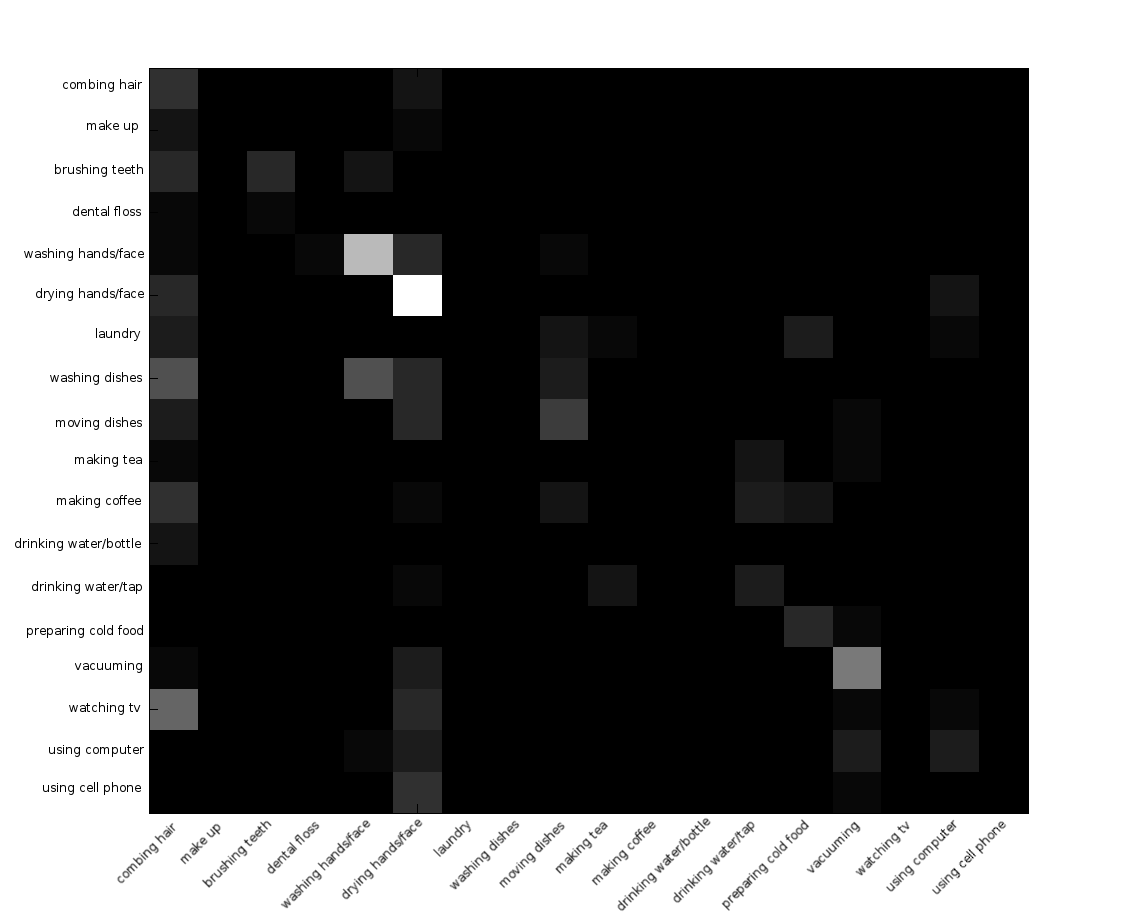
\includegraphics[width=10.0cm]{figures/confn2-labels.png}}}
		   \caption{Confusion matrix for RSTP+OCC using detected active and
       passive objects}
  \label{fig:teaser}
  \end{center}
  \end{figure}
	As seen in Figure 3, our method has particularly good
  performance for activity types 5 and 6 (``combing hair'' and ``drying
  hands/face'', respectively). Some activity types on which our method does
  poorly are 10 and 11, which are ``making tea'' and ``making coffee'',
  respectively (see Table 1 for a full listing of activity types present in
  the ADL dataset). Since the two activity types are similar in the sense that
  they involve the same active objects, it is not
  unexpected that a recognition system would confuse them often.
  
  To illustrate the improvement on accuracy obtained from using a pool of
  biased partitions, we created 3 separate pools containing 4-level
  partition schemes of each bias type and
  repeatedly ran the cross-validation experiment, adding additional
  partitions to each pool between runs. The pool containing partitions of
  bias type 3 consistently outperformed the pool of bias type 2, which
  consistently outperformed the unbiased pool. The
  results from this experiment are depicted in figure 4. We were initially
  surprised to find that increasing pool size can
  sometimes negatively impact overall classification accuracy, however we
  believe this is due to the inherent bias between the training and the test
  data. In other words, sometimes a partition scheme with small training error
  on the train data that gets selected during a round of boosting can have a
  larger training error on the test data. A similar behavior was discovered
  in the case of boosting spatial pyramids for 2D image recognition
  \cite{Jiang12}.
 
  \begin{figure}[t]
		\begin{center}
			%\fbox{\rule{0pt}{2in} \rule{0.9\linewidth}{0pt}}
			  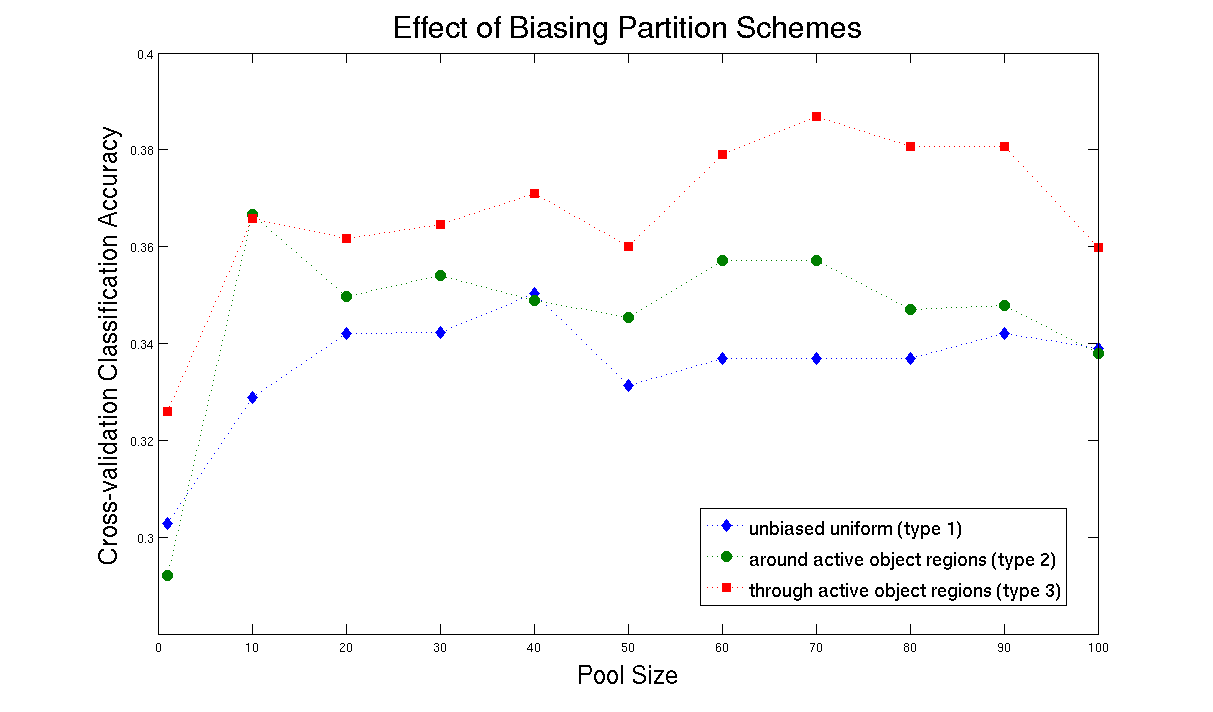
\includegraphics[width=1.0\linewidth]{figures/biaseffect.png}
		\end{center}
		   \caption{Effect of using biased partition schemes. The pool
       containing type 3 biased partition schemes consistently outperforms
     the other pools.}
				\label{fig:long}
				\label{fig:onecol}
	\end{figure}
  
  To further support our claim that 4-level pyramids of bias type 3 tend to be most
  discriminative, we created a heterogeneous pool containing partition
  schemes of
  several different types. Specifically, the heterogeneous pool contains 30 2-level
  partitions of each bias type, 30 3-level partitions of each bias type, and
  30 4-level partitions of each bias type, for a total of 270 partitions.
  We generated 20 random 50/50 train/test splits, fixed the number of
  boosting rounds to 5, and observed which types of partitions were most
  often selected during boosting rounds.
  We found that partition schemes with more levels tend to get selected more
  often during boosting rounds.
  Specifically, we found that 2-level pyramids of bias type 3 were selected
  21\% of the time, 3-level pyramids of bias type 3 were selected 19\% of
  the time, and 4-level pyramids of bias type 3 were selected 37\% of the
  time. 2-level and 4-level unbiased pyramids were never selected. Thus,
  biased partition schemes that cut through regions that tend to contain
  active objects are clearly more discriminative than other types of
  partition schemes, especially those which are unbiased.
	
\section{Conclusion and Future Work}
	We have presented an application of the well-known boosting framework
	with results for an
  egocentric activity recognition task that improve upon the current state of
  the art.
	Our main novel contribution is a method for generating biased partition
	schemes based on observations of active object locations throughout the
  training data (Object-Centric Cuts).
	Future work could potentially incorporate different types of biases when generating
	partitions. The ADL dataset also includes annotations for hand positions,
	which we have incorporated implicitly through our generation of biased partitions
	biased relative to regions which tend to contain active objects. However,
	it could be possible to incorporate explicit information given by hand
	positions to obtain better classification results.
	The partitions we focus on contain cuts that are
  planar and axis-aligned (we consider random shifts but not random
  rotations, and we do not consider non-planar splits),
  but it is possible to carve up the
	video volume in more advanced non-linear ways. Such a method would involve more
	sophisticated computational geometry, but may yield a more discriminative
	partitioning scheme that could lead to better classification accuracy.
\bibliography{egbib}
\end{document}
